\chapter{Columnar Storage}
\label{c:columnar-storage}

In this chapter, we explore the application of columnar data structures for different storage components of  \gls{gdbms}s to meet the desiderata we outlined in Chapter~\ref{c:guidelines}. 

Section \ref{sec:vertex-property-columns} describes the design of columns to store vertex properties, called \emph{vertex columns}, and a new compact vertex ID scheme that accompanies the design. In Section \ref{sec:edge-property-columns}, we start by describing two columnar storage designs to store edge properties and their pros and cons. Then, we propose our final design, \emph{single-directional property pages}, that is a sweet spot between the earlier two designs and the one we use for storing edge properties. Similar to Section~\ref{sec:vertex-property-columns}, we describe a novel and compact edge ID scheme that accompanies our design of single-directional property pages. In Section~\ref{sec:adjacency-lists}, we briefly describe the existing structure of adjacency lists in GraphflowDB that is implemented as \gls{csr}, which is already a variant of columnar data structure and stores adjacent edges and neighbour vertices of a particular vertex in contiguous memory locations. In Section~\ref{sec:single-cardinality-cols}, we look for better ways of storing edges and hence, describe a storage optimization that involves storing edges with cardinalities 1-1, 1-n, n-1 in vertex columns instead of using heavy-weight \gls{csr} columnar structure. We address how to compress the data stored in these columnar structures in Chapter~\ref{columnar-compression}. Finally, Section~\ref{summary} summarizes our new storage layout for storing edges and properties of the graph data.
%Section~\ref{sec:storage-optimizations} describes several storage optimizations to the adjacency lists to reduce the system's memory footprint without sacrificing query performance, using different type of structure that may exist in input graphs that we observed in Guideline~\ref{gdln:graph-schema}.

\section{Columnar Storage for Vertex Properties}
\label{sec:vertex-property-columns}

\begin{figure}
	\hfill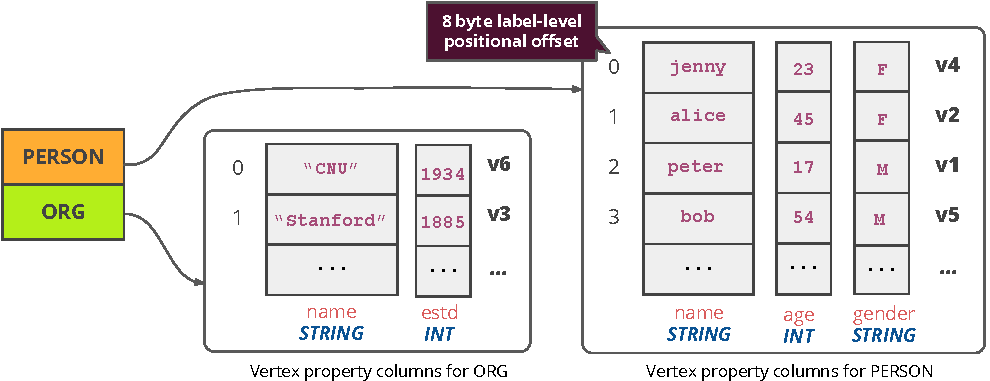
\includegraphics[scale=0.85]{img/vpcols}\hspace*{\fill}
	\caption{Vertex columns for the graph in Figure~\ref{fig:runn}.}
	\label{fig:vpcols}
\end{figure}

Columnar data-structures can be directly used for storing vertex properties. Let $lv_1, lv_2, ...$ be the vertex labels in a graph. Let $p_{i,1},  p_{i,2}, ... p_{i, n}$ be the structured vertex properties of $lv_i$, each with a specific datatype $d_{i,j}$. We define a \emph{vertex column} for each $p_{i,j}$, having a fixed data type $d_{i,j}$. Each column stores the value of a single property $p_{i,j}$ for all vertices having label $lv_i$ at consecutive locations. All property values of a particular vertex $v$ with label $lv_i$ is located at the same positional offset in the column for each $p_{i,j}$. 

% reading a property.

Ideally, the property value of a vertex should directly be read using the ID of the vertex as the positional offset in the column. However, \gls{gdbms} typically gives globally unique 8-byte consecutive IDs to all the vertices in the system, irrespective of their labels. That means ID 0 can be given to a vertex with label \texttt{PERSON} and 1 to a vertex with label \texttt{ORG} and 2 to another vertex \texttt{PERSON} etc. We cannot use this ID scheme as the positional offset for the above design. One possible solution is to maintain a map for each label, from each vertex $v$'s \enquote{global} ID to a \enquote{local} label-level positional offset, which is unique only among all vertices with the same label as $v$. This requires extra storage for maintaining the map and one level of indirection when accessing the vertex properties. Instead, we adopted an ID scheme where each vertex is identified by a \emph{\textbf{(vertex label, label-level positional offset)}} tuple in the system in place of global vertex ID. This allows direct access to the properties by using the local positional offset which now is part of the vertex ID. However, using this new vertex ID scheme requires materializing 2 pieces of information in the adjacency lists - a vertex label and a local positional offset, compared to a single global vertex ID. This may increase the memory overhead  if the local positional offsets and the global vertex ID are of the same size. However, we will show in Section \ref{sec:storage-optimizations} that we can often avoid storing the vertex labels with vertex IDs and even save space by using fewer bytes for local positional offsets than the bytes needed by the global vertex IDs.

For reference, Figure~\ref{fig:vpcols} shows a set of vertex columns for our example graph in Figure~\ref{fig:runn}. It has 2 set of columns, one for each vertex label, with a column for each structured property of the label. The global vertex IDs on the right of the set of columns of a vertex label indicates the positional offset at which the properties of a particular vertex are located in the columns of a particular label. For instance, the properties of vertex \texttt{v2} appear at offset $1$ in columns of \texttt{PERSON}. By the new vertex ID scheme, \texttt{v2} is identified as \texttt{PRESON:1}. 

% updates.

Recall from Guideline~\ref{gdln:vertices-unordered} that in general, reading the properties of vertices (specifically when reading the properties of neighbors of a vertex) cannot be localized without prohibitive replication. In light of this guideline, we adopt a simple and efficient additions and deletion scheme for of vertex properties and vertices. Deleting a single property of vertex $v$ is handled by setting the property at $v$'s positional offset to NULL. Deleting $v$ is handled by removing all the outward and inward edges of $v$, setting all of $v$'s properties to NULL, and adding $v$'s positional offset to a list of ``recycled'' offsets. When a new vertex $v$ is added, the system generates an ID by using a recycled offset if one exists or gives a new consecutive positional offset (i.e., increments the maximum positional offset by 1). Updating $v$'s property is handled by overwriting the value in the property column for $v$'s positional offset. All of these operations are very efficient involving only random access to different locations in columns.

\section{Columnar Storage for Edge Properties}
\label{sec:edge-property-columns}

Recall from Guideline~\ref{ssec:edges-ordered} that edges and their properties are read by the \texttt{JOIN} and \texttt{PROPERTY READER} operators, respectively, in the order they appear in the adjacency lists. \gls{gdbms}s store the edges, i.e the (edge ID, neighbour vertex ID) pairs, consecutively in adjacency lists, through double indexing. Ideally, edge properties should also be stored in the same order. In this section, we begin by presenting two columnar storage designs for storing edge properties which can be seen as opposite ends of a design spectrum. The first design, {\em edge columns}, is optimized for \emph{storage} and does not replicate the edge properties. The second design, {\em double-indexed property lists}, is optimized for \emph{performance} through double indexing of the edge properties, similar to edges in the forward and backward adjacency lists. We then describe a third design, {\em single-directional property lists}, that can be seen as a sweet spot between the previous two designs, which localizes the reads in one direction without any replication. However, this natural third design has several limitations, that we address in our final design, {\em single-directional property pages}, which is adopted in GraphflowDB. 

% However, this also requires double indexing, which is expensive as each property needs to be replicated. 
\begin{figure}
	\vspace{-20pt}
	\hspace*{-20pt}
	\begin{subfigure}{0.45\textwidth}
		\vspace{14pt}
		\centering
		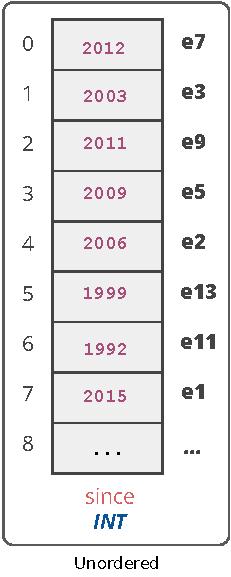
\includegraphics[scale=0.69]{img/sol1}
		\captionsetup{justification=centering}
		\vspace{12pt}
		\caption{Edge Columns}
		\label{fig:sol1}
	\end{subfigure}
	\begin{subfigure}{0.55\textwidth}
		\centering
		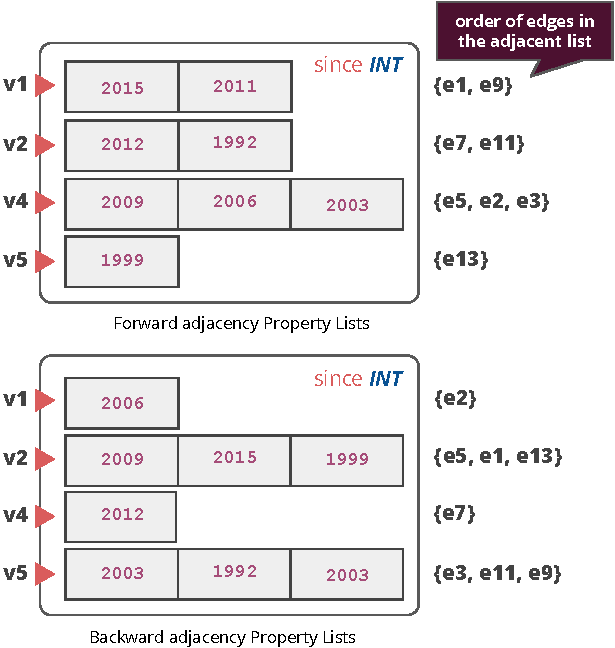
\includegraphics[scale=0.69]{img/sol2}
		\captionsetup{justification=centering}
		\caption{Double-indexed Property Lists}
		\label{fig:sol2}
	\end{subfigure}
	\captionsetup{justification=centering}
	\caption{Storing edge properties of \texttt{FOLLOWS} edges in the Edge Columns and Double-indexed Property Lists.}
	\label{fig:sol1and2}
\end{figure}

\subsection{Edge Columns and Double-Indexed Property Lists}
\label{sec:edge-cols-prop-lists}

\noindent {\bf Edge Columns (Non-sequential reads, no replication):} One possibility is to use the columnar storage design similar to that for storing the vertex properties. That is, we have one edge column for each $q_{i,j}$, where $q_{i,j}$ is a structured property of edge label $le_i$. Edges in the system with this solution can be identified as \emph{(edge label, label-level positional offset)}. However, such a design would not localize the properties of the edge according to their appearance in the adjacency lists, so cannot provide sequential reads when reading the edge properties. Figure~\ref{fig:sol1} shows how this particular design would look like. The figure shows a column storing property \texttt{since} of \texttt{FOLLOWS} edges. The property values are not ordered. For our example, the forward adjacency list of \texttt{v4} contains edges \texttt{e5}, \texttt{e2} and \texttt{e3}, whose \texttt{since} property values (at positional offsets 3, 4 and 1) are not stored consecutively in the edge column. 

\noindent {\bf Double-Indexed Property Lists (Sequential reads in both directions, 2x replication):} An alternative solution is to directly mimic the storage of the adjacency lists for storing the edge properties in both the directions. For each vertex $v$ that has edges with a label $le_i$, and each $q_{i,j}$, we store the edge properties in the \emph{forward property lists} and \emph{backward property lists}. This provides sequential read of properties. For example, a query that is reading the forward (backward) adjacency list of $v$ can read the edge property values of the edges sequentially from the forward (backward) property list of $v$. Figure~\ref{fig:sol2} shows the forward and backward property lists for edgel label \texttt{FOLLOWS} in our example graph in Figure~\ref{fig:runn}. However, this design requires replicating each edge property twice. In addition, if the original adjacency lists are sorted, then all the property lists need to be sorted too in the same way, which would make updates slower. 

\subsection{Single-directional Property Pages}
\label{sec:single-directional-property-pages}

\begin{figure}
	\hfill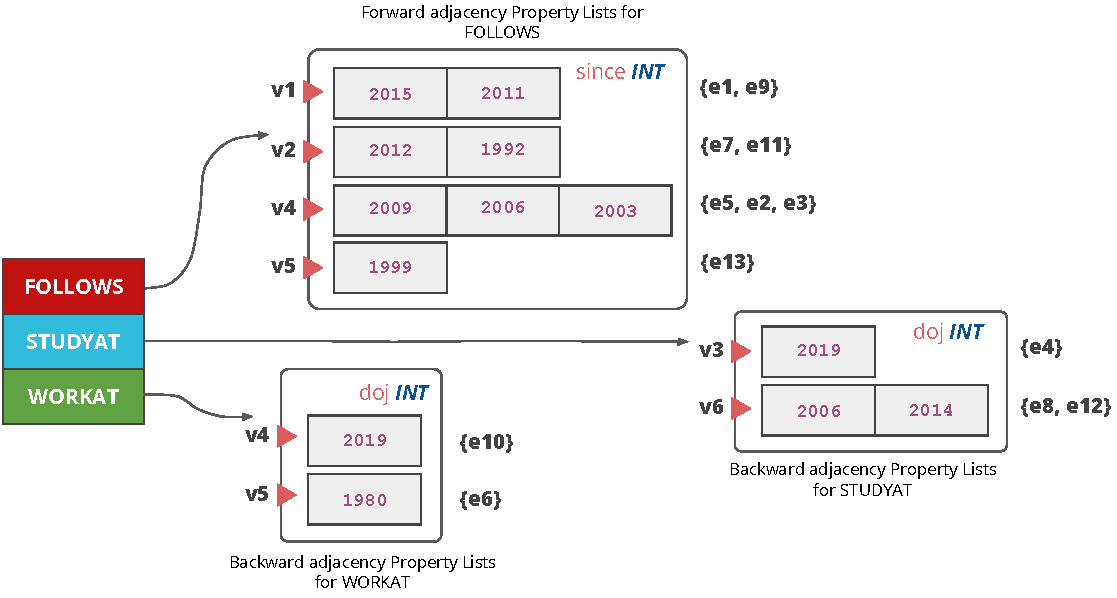
\includegraphics[scale=0.78]{img/single-dir-prop-list}\hspace*{\fill}
	\captionsetup{justification=centering}
	\caption{Single-directional Property Lists}
	\label{fig:single-dir-prop-list}
\end{figure}

A natural middle ground between edge columns and double-indexed property lists is to store only one of the forward or the backward property lists. We call this design \emph{single-directional property lists}. Suppose the system indexes the properties of the edges with label $le_i$ in the forward direction. Then, the edge properties can be read sequentially if edges are read from the forward adjacency lists. However when reading the edges in the backward direction, then the edge properties will not be sequential. Figure~\ref{fig:single-dir-prop-list} shows the single-directional property lists for storing the edge properties of the example graph in Figure~\ref{fig:runn}. In the example, edge properties of \texttt{FOLLOWS} and \texttt{WORKAT} labels are stored in the forward property lists, while for \texttt{STUDYAT}, the edge properties are in the backward property lists. In this design, reading the edges having label \texttt{FOLLOWS} or \texttt{WORKSAT} in the backward direction requires that given the ID of an edge $e$, the system is able to locate the positional offset of $e$ in the forward direction to access its properties from forward property lists. This requires a new edge ID scheme that is structurally similar to our new vertex ID scheme described previously. Specifically, the conventional globally consecutive edge IDs cannot be used to access the properties quickly as they do not contain information about positional offsets. We next describe a new edge ID scheme to achieve this. Then we talk about some important limitations of single-directional property lists, which we address by further modifying this design.

\begin{figure}
	\hfill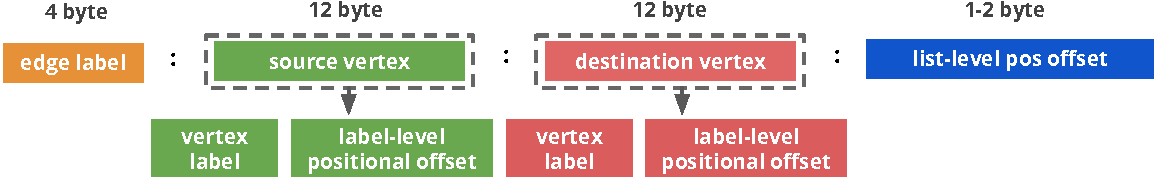
\includegraphics[scale=0.78]{img/edge-scheme}\hspace*{\fill}
	\captionsetup{justification=centering}
	\caption{Components of the new edge identification scheme.}
	\label{fig:edge-scheme}
\end{figure}

To access a property of an edge $e$ having label $le_i$, we need 3 pieces of information; 1) $q_{i,j}$; 2) source vertex if the $q_{i,j}$'s values are stored in the forward property lists, else destination vertex; and 3) the list-level positional offset of $e$ in that property list. For instance, in figure~\ref{fig:single-dir-prop-list}, \texttt{since} property of $e2$ can be accessed knowing $v4$ (source vertex of $e2$) and offset of $e2$ in $v4$'s forward property list, i.e 1. We adopt a new edge identification scheme that identifies the edge in the system by a tuple having 4 components: \textbf{\emph{(edge label, source vertex, destination vertex, list-level positional offset)}}. In our new scheme, the $e2$'s ID will be given as \texttt{FOLLOWS:v4:v1:2}, where $v4$ and $v1$ are the source and destination edges of $e2$. These new edge ID scheme are pivotal in achieving compact representation of edges and vertices in adjacency lists too. Most of the components of our new edge ID need not be stored in the adjacency lists and the edge ID can be constructed during query execution by reading as few as only the neighbour vertex's local positional offset in the property list.

\noindent {\bf Limitation of single-directional property lists:} Though single-directional property lists are a good middle-ground solution, it has an important limitation. Suppose that the property list for property $q_{i,j}$ of edge label $le_i$ is indexed in the forward direction. If the original adjacency lists are sorted, any insertion or deletion can change the positional offset of a large number of, possibly all the edges in the adjacency list. As such, keeping the edge ID mutable and requiring it to change frequently induces added complexity in maintaining consistency of edge IDs in the system. Suppose an edge is inserted to the beginning of $v$'s forward adjacency list $L_f$. This requires first calculating a map of old and new positional offsets of the edges in $L_f$, then searching through each backward neighbour of $v$ and finding each edge in it's backward adjacency list and updating its positional offset. The problem is further escalated if there are other secondary indexes in the system on the effected edges. A similar problem exists when an edge is deleted. If the original edges are not sorted, then insertions can be handled easily but handling deletions is challenging. The system has two options for deletions. First, the system can directly delete the edge $e$, which again can change the positional offsets of as many as $|L_f|$ edges. Instead, the system can thumbnail $e$'s positional offset and recycle $e$'s positional offset as was described for vertex deletions. However, this is also expensive. In contrast to keeping a single list of recycled IDs as in vertex columns, the system now needs to keep track of recycled positional offsets for each vertex, so up to $|V|$ many recycled IDs list.

\begin{figure}
	\hfill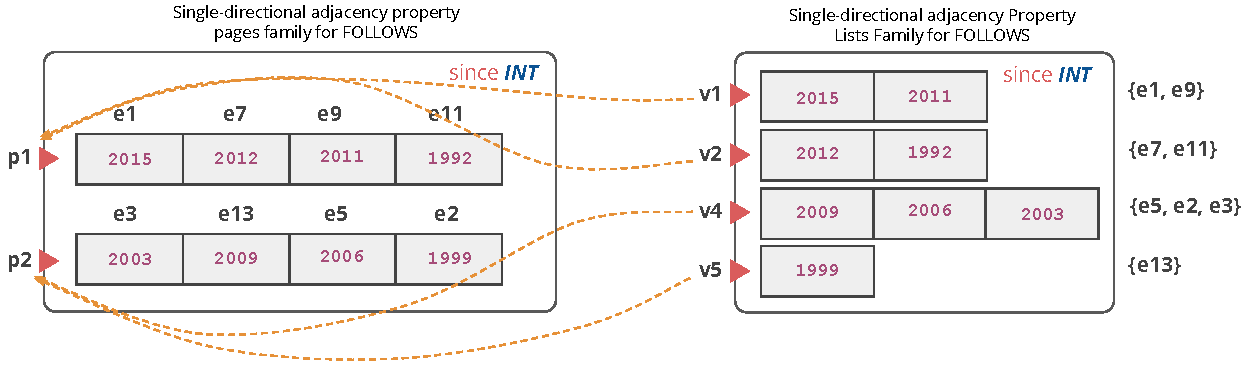
\includegraphics[scale=0.78]{img/paged}\hspace*{\fill}
	\captionsetup{justification=centering}
	\caption{Mapping single-directional property lists to single-directional property pages for since property in Figure~\ref{fig:runn}.$n=2$.}
	\label{fig:paged}
\end{figure}

\noindent {\bf Single-directional property pages:} To address the above limitation, we take $n$ property lists (by default 64) and store their properties together, in a  \emph{property page}. Properties in a property page are not necessarily stored consecutively to preserve the ordering of property lists. However, because we use a small value of $n$ and adjacency lists of many vertices are short in many real world datasets, these properties are stored in close-by memory locations thereby ensuring good cache locality while accessing. We do not sort these pages when the original adjacency lists are sorted and keep a recycled ID list for each page, avoiding the cost of sorting and the maintenance of list-level recycled ID lists. We can use the same edge ID scheme we described above, except the positional offsets now identify the properties of edges in property pages, instead of property lists. Suppose again that the property $q_{i, j}$ is stored in the forward direction (properties of $n$ lists are grouped together). Given an edge $e$ in the scheme from Figure~\ref{fig:edge-scheme}, we can take the source vertex's label-level positional offset and divide it by $n$ to identify the page in which $e$'s $q_{i, j}$ property is. Within this page, the property can be accessed with a single lookup using the positional offset of $e$.

%The mapping from a property list to its corresponding page is straightforward. Single-directional property list for vertex $v$ and property $q_{i,j}$ maps to the $i$th page for property $q_{i,j}$, where $i$ is mod $n$ of $v$'s local positional offset. The benefit of using pages comes from it being unordered. This makes new edge insertions easy as now, the new edge properties get appended into their respective pages or recycle the location of an already deleted edge, similar to how insertions happen in vertex columns. 

Figure~\ref{fig:paged} shows the mapping of a single-directional property lists to single-directional property pages for $n=2$. The single-directional property pages for FOLLOWS edges has two pages that stores the property values from vertex groups $(v1,v2)$ and $(v3,v4)$ respectively, assuming that the local positional offset of $vi$ is $i$ and $pi$ is the $i$th property page for \texttt{since} property. 
%The value of $n$ is chosen such that edges' property values are not too far apart from each as they were stored in %the property lists. This reduces the cache miss to occur with \emph{each} access of a value in a page. Hence, the value of $n$ is dependant on 3 factors: 1) the cache line size; 2) width of an element in the page, and 3) the average number of edges in the adjacency lists. Ideally, the value of n is optimum in the range $[32, 512]$. 
In Section~\ref{exp:property-pages}, we show that the single-directional property pages is similar, about 1.2x slower, in performance to single-directional property lists in read-heavy stress tests and about 2.5x faster than using edge columns. 

\section{CSR Adjacency Lists}
\label{sec:adjacency-lists}

\begin{figure}
	\hspace{-15pt}
	\hfill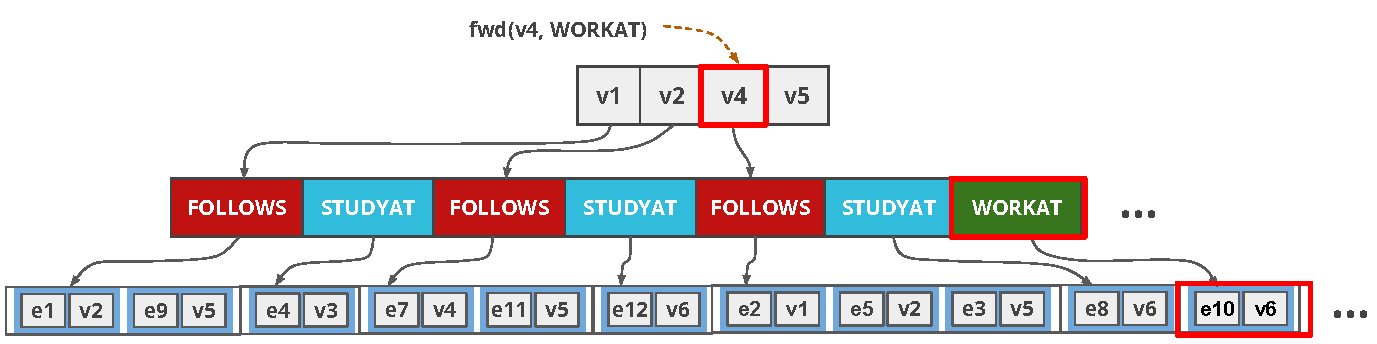
\includegraphics[scale=0.75]{img/adjlists}\hspace*{\fill}
	\captionsetup{justification=centering}
	\caption{Forward adjacency lists implemented as a 2-level CSR structure for the example graph.}
	\label{fig:adjlists}
\end{figure}

In GraphflowDB, the adjacency lists of a vertex are further partitioned by the adjacent edge's label and sorted by neighbour vertex's ID to support matching cyclic queries that need to join multiple query edges at a time in a single \texttt{JOIN} operation. We implement the adjacency lists in a 2-level \gls{csr} structure. The \gls{csr} can be thought of as a columnar data structure that stored multi-value attributes. Figure~\ref{fig:adjlists} shows the physical data layout of forward adjacency lists in our example graph. The adjacency list of each vertex is indexed by its vertex ID, which is the list of sequential positional offsets, for each label. This is implemented as an array of offsets to the first level of \gls{csr} that contains one entry per edge label that a particular vertex has edges of. Similarly, this first level of \gls{csr} holds offsets to the next level of the \gls{csr} that consists of a list of (adjacent edge, neighbour vertex) pairs, that are sorted by the neighbour vertex ID. Each sublist in the final \gls{csr} is the set of edges of a particular vertex and having a particular label. This sublist sits at the depth of 2 in the hierarchy and hence, can be accessed by 2 indirections.

GraphflowDB represents edge and vertex ID as 8 byte values which means that each edge in the adjacency lists has the payload of 16 bytes. Our new vertex and edge ID scheme compacts this representation. As show in Section~\ref{sec:storage-optimizations}, the payload for each edge in the adjacency lists can be significantly reduced by exploiting the structures in graph that we describe in Guideline~\ref{gdln:graph-schema}. With our set of optimizations, we end up reducing the size of this payload to only 4 bytes at times.

\section{Vertex Columns for Single Cardinality Edges}
\label{sec:single-cardinality-cols}

\begin{figure}
	\hfill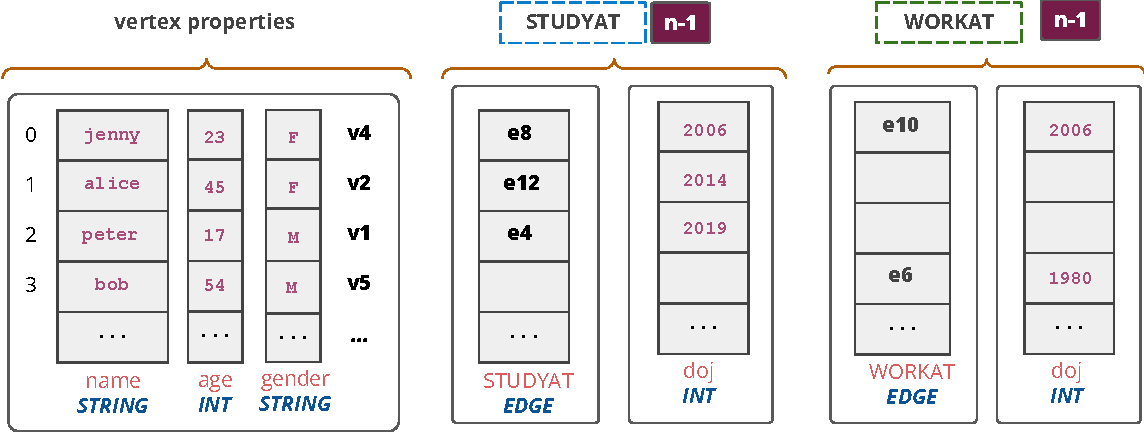
\includegraphics[scale=0.78]{img/single-cardinality-cols}\hspace*{\fill}
	\captionsetup{justification=centering}
	\caption{Storage of edges having single cardinality edge label \texttt{STUDYAT} and \texttt{WORKAT} as special property of \texttt{PERSON}. \hspace{\textwidth} Properties of these edges are also stored in vertex columns of \texttt{PERSON}.}
	\label{fig:single-cardinality-cols}
\end{figure}

When an edge label has 1-1, 1-n, n-1 cardinality, then the vertices can have at most one edge of that label in at least one direction. We refer to these edges as {\em single cardinality edges}. For instance, in our Figure~\ref{fig:runn} example graph, edge labels \texttt{STUDYAT} and \texttt{WORKAT} have cardinality \texttt{n-1}, i.e., a \texttt{PERSON} vertex can have at most one \texttt{STUDYAT}'s and \texttt{WORKAT}'s edge (in the forward direction). In this, the vertices of \texttt{ORG} label can still have multiple \texttt{STUDYAT} and \texttt{WORKAT} inward edges. Therefore, instead of storing these edges of single cardinality edge labels in the adjacency lists in last level of the 2-level \gls{csr} structure, we can store them as a \emph{property} of source or(and) destination vertex and directly access them using the positional offsets of the source or(and) destination vertex of the edge. This both saves space, as we do not need to store the \gls{csr} offsets, and we can directly access these edges with 1 instead of 2 random lookups in the rudimentary 2-level \gls{csr}. Similarly, the properties of these edges can also be stored in vertex columns as a property of either the source or destination vertex. Thus, we do not need page-level positional offsets for these single edges since the edge property can be accessed using the source or destination vertex's positional offset, similar to how the edge is accessed. Figure~\ref{fig:single-cardinality-cols} shows the edges of edge label STUDYAT and WORKAT, from our example graph, and their properties being stored as the special property of vertex type \texttt{PERSON}.

%Benefits of storing edges as special vertex properties is two-fold, Figure~\ref{fig:single-cardinality-cols} shows the STUDY AT edges stored as the special properties of PERSON vertices. Moreover, the properties of such an edge $e$ can also be stored in structures similar to the vertex columns, instead of single-directiional property pages. These properties are hence, accessed by vertex $v$'s local positional offset, instead of page-level positional offset, where $v$ is the vertex whose special property the edge is. Thus, we do not need page-level positional offsets for the edges of single cardinality edge labels.


\section{Summary}
\label{summary}

\begin{table}[t!]
	\centering
	\bgroup
	\setlength{\tabcolsep}{10pt}
	\def\arraystretch{1.3}%  1 is the default, change whatever you need
	\begin{tabular}{ |c|c|c| } 
		\hline
		\multicolumn{2}{|c|}{\textbf{Data}} & \textbf{Columnar data structure} \\
		\hline \hline
		\multicolumn{2}{|c|}{Vertex Properties} & Vertex columns \\
		\hline \hline
		\multirow{4}{60pt}{Edge Properties} & 1-1 & Vertex column of either source or destination vertex label\\
		\cline{2-3}
		& 1-n & Vertex column of destination vertex label\\
		\cline{2-3}
		& n-1 & Vertex column of source vertex label\\
		\cline{2-3}
		& n-n & Single-directional property pages \\
		\hline \hline
		\multirow{7}{60pt}{Edges} & \multirow{2}{20pt}{1-1} & Vertex columns of source vertex for forward edge \\
		&& Vertex column of destination vertex label for backward edge \\
		\cline{2-3}
		& \multirow{2}{20pt}{1-n} & CSR Adjacency lists for forward edge \\
		&& Vertex columns of destination vertex label for backward edge \\
		\cline{2-3}
		& \multirow{2}{20pt}{n-1} & Vertex column of source vertex label for forward edge \\
		&& CSR Adjacency lists for backward edge \\
		\cline{2-3}
		& \multirow{1}{20pt}{n-n} & CSR Adjacency lists for forward and backward edges \\
		\hline
	\end{tabular}
	\egroup
	\captionsetup{justification=centering}
	\caption{Our Columnar data structures and the component of the property graph for which they are used. The storage classification of edge properties and edges is further dependant on that edge's label's cardinality.}
	\label{tbl:summ}
\end{table}

Table~\ref{tbl:summ} presents the summary of our storage. For each of the component in the property graph data, we classify as to which data structure they are stored in. 
